
%----------------------------------------------------------------------------
\chapter{Preliminaries}
%----------------------------------------------------------------------------

In this chapter, we revisit the background knowledge on graph-based modeling, and graph pattern matching. We also introduce the used terminology as it is crucial in the following chapters. At the end of the chapter, we show how the concepts of graph pattern matching can be extended to run over distributed systems.

\section{Graph-based modeling}

Structural and behavioral modeling of systems is often done using graphs. 
Graphs are useful as they are easy to understand, intuitive to use, and lots of existing algorithms can be used to process them. 
As our model-based approach introduced in the framework relies on graphs as a representation, in this section, graph-based modeling is presented.

A directed graph consists of a set of nodes and a set of edges, where edges are ordered pairs of two nodes. An edge has a \emph{source} node and a \emph{target} node. 
Graphs can be extended to represent models by adding extra information, such as:
\begin{itemize}
	\item assigning a type to each node
	\item assigning a type to each edge that specifies the types of the source and the target node
	\item supplying nodes with attributes and attribute values (e.g.\ name)
\end{itemize}


\begin{figure}[H]
	\begin{center}
		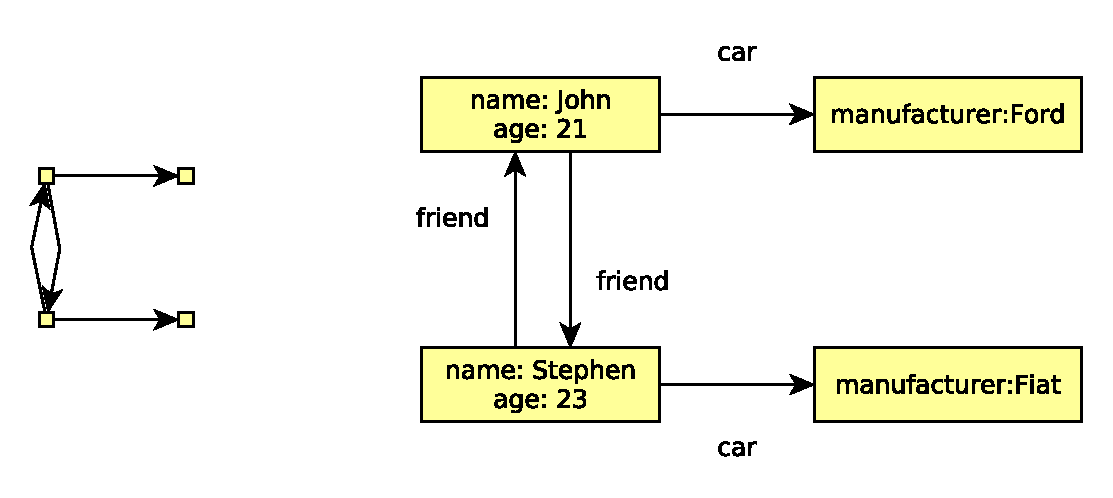
\includegraphics[width=\textwidth]{figures/graphs.pdf}
		\caption{Basic graph (left), and extended (right) }
		\label{fig:graphs}
	\end{center}
\end{figure}

To be consistent with the terminology used in software engineering, we also use the term \emph{object} for a typed node with attributes and \emph{reference} for a typed edge. 

A metamodel is a model, that defines how the graph model of a system is built up:
\begin{itemize}
	\item what type of objects exist
	\item what kind of attributes can a node of a certain type have
	\item what type of references exist and what type of object can be its source and target node
	\item multiplicity restriction for references and attributes
	\item hierarchical relationship between types
\end{itemize}

\autoref{fig:metamodel} shows some of these concepts. The upper part is a metamodel, and the lower is an instance model, that satisfies the rules defined by the metamodel: There can be 3 types of objects: \texttt{ModelElement}, \texttt{Train} and \texttt{RailRoadElement}. All instances of \texttt{ModelElement} has an \texttt{id}. Both of \texttt{Train} and \texttt{RailRodeElement} are a subtype of \texttt{ModelElement} which means, that each instance of the subtype works as an instance of the supertype as well.
\begin{figure}[h]
	\begin{center}
		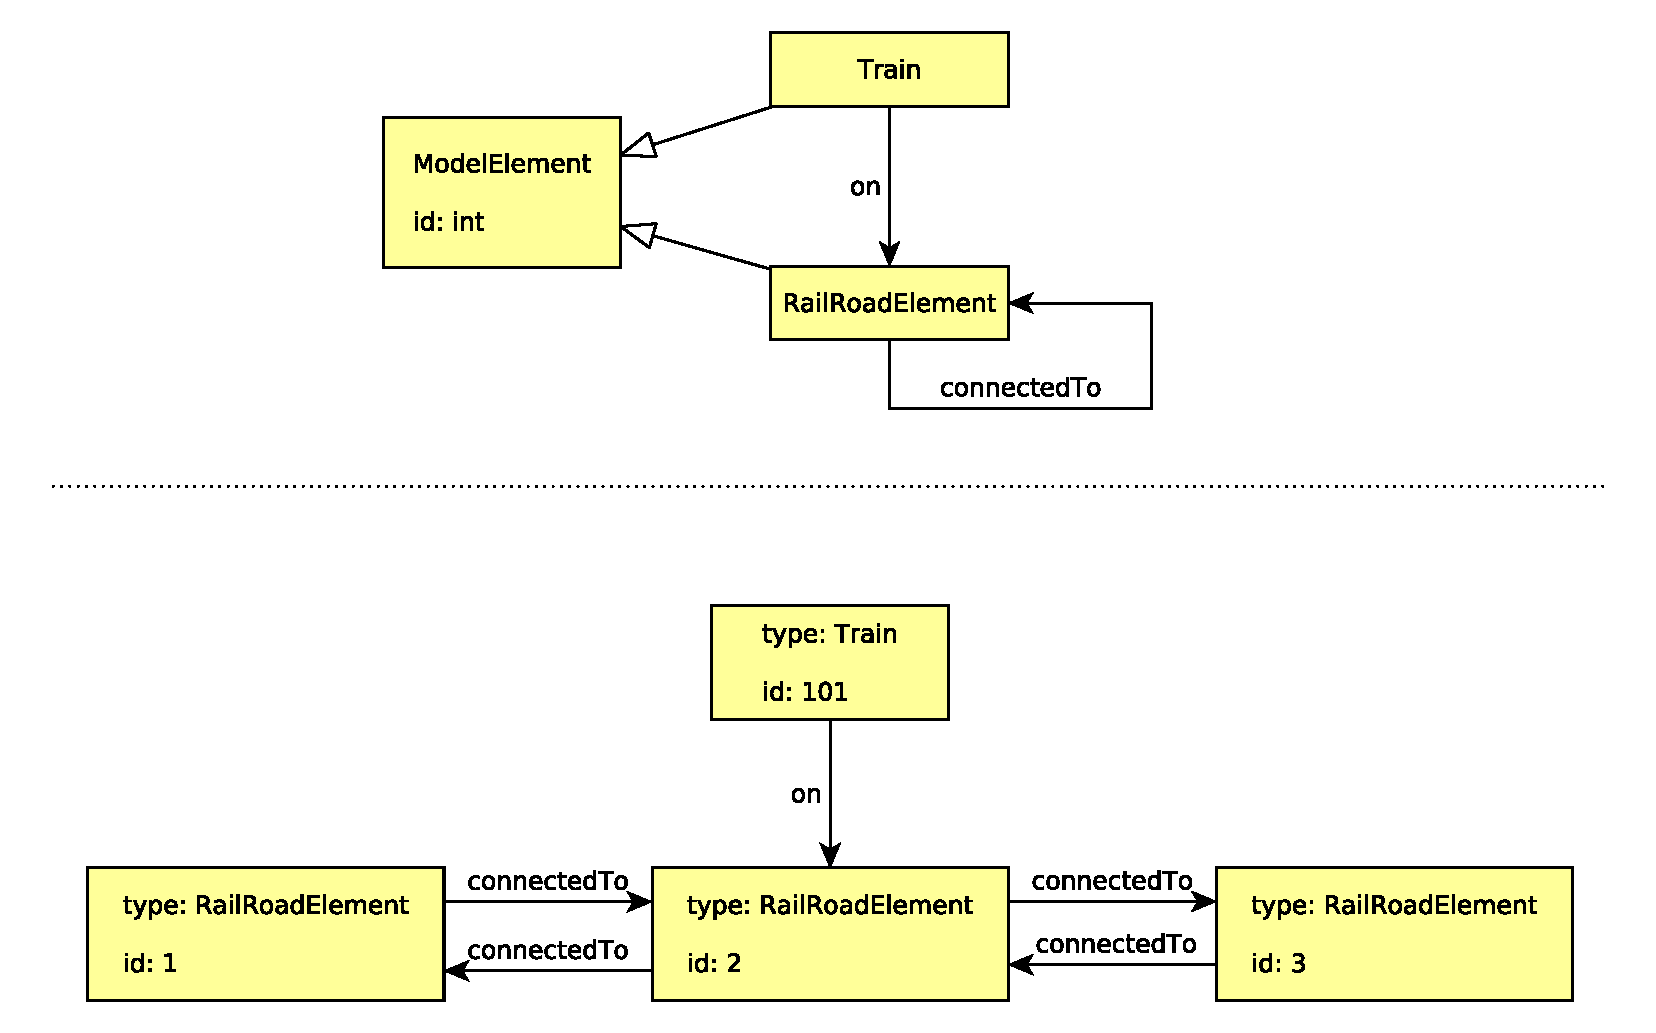
\includegraphics[width=\textwidth]{figures/metamodel.pdf}
		\caption{ Example of a metamodel and an instance model }
		\label{fig:metamodel}
	\end{center}
\end{figure}


\section{Domain and runtime modeling}

In this framework, we use graph-based models to represent the current state of the system. 
The state and the operating context of the system are captured in a model called the \emph{live model} or \emph{runtime model} \cite{Szvetits2013, DBLP:journals/computer/BlairBF09}.
It is updated with sensor data and information from other sources, so the model captures the physical system's latest known state.
This model is used for runtime verification.
While the model is being continuously updated it is also analyzed using graph pattern matching to find parts of the model that may imply error in the system.

An example of a live model is depicted in \autoref{fig:live-models}. As the train with \texttt{id}=105 is moving from the segment with \texttt{id}=1 to segment with \texttt{id}=2, the appropriate railway sensors send updates to the model, which is modified to represent, that the train is on an other segment.




\begin{figure}[H]
	\begin{center}
		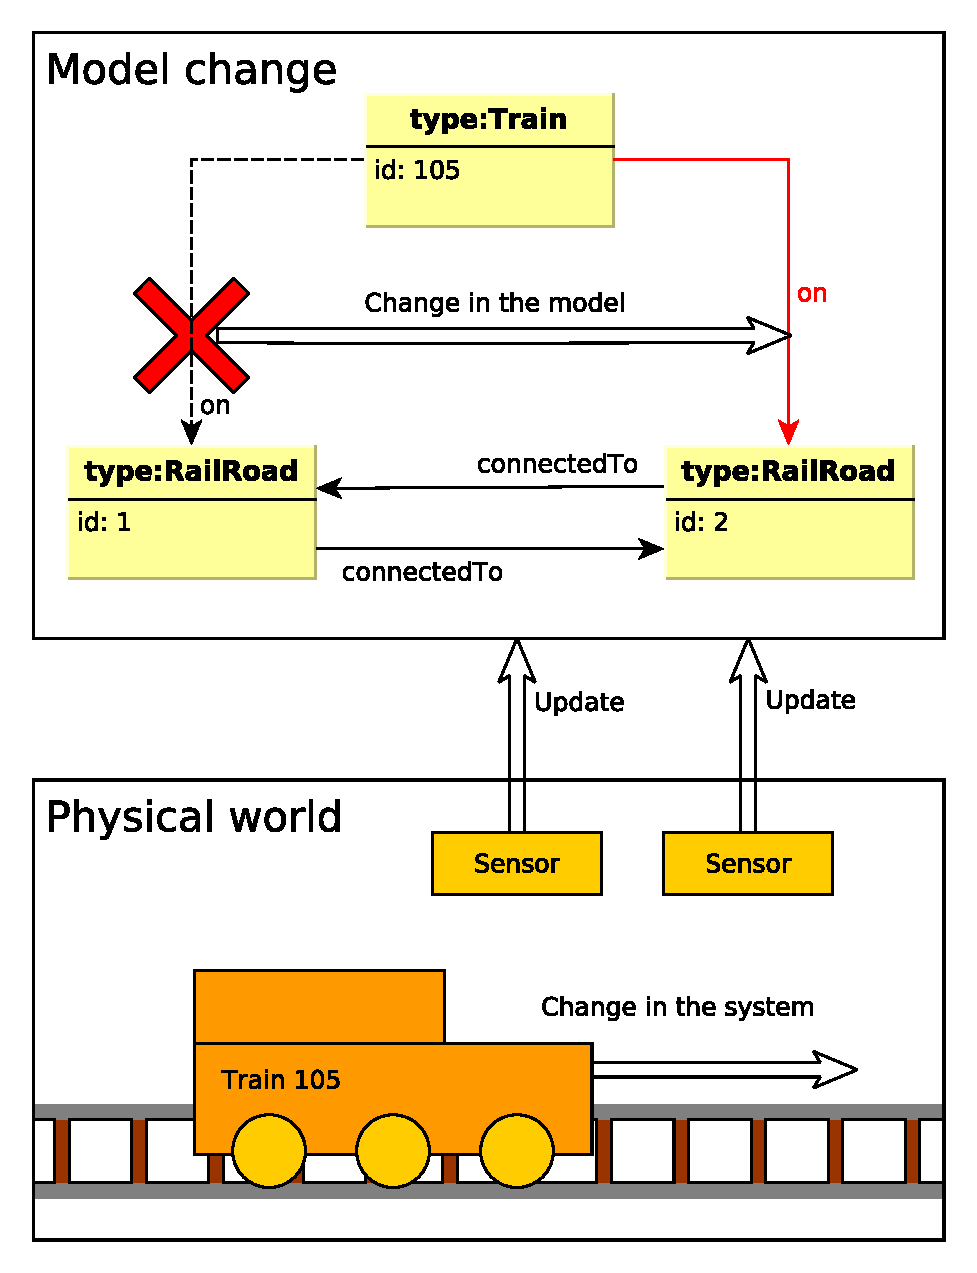
\includegraphics[width=0.7\textwidth]{figures/live-models.pdf}
		\caption{Live model updating}
		\label{fig:live-models}
	\end{center}
\end{figure}

\section{Foundations of graph pattern matching}
\label{section:gpmc}

\todo{Marci tanácsait bevezetni, ha frissebb leszek}
\todo{Tetszőleges kifejezéssel lehet gráf patternt adni, viszont a viatra és a local search miatt adott egy értelmes formához kötni magunkat}

The goal of graph pattern matching is to find all subgraphs of a graph meeting a certain criteria, defined by a \emph{graph pattern}.

We define the domain of an extended graph as the union of 
\begin{itemize}
	\item the set of the vertices of the graph
	\item and the set of data values (Strings, numbers, boolean values, and enumeration literals), that can be assigned to the attributes of its vertices
\end{itemize}

A \emph{graph pattern} is a predicate, and its  domain is the domain of the extended graph.
A \emph{pattern match} is a tuple of elements from the graph domain, that satisfies the predicate.
A pattern's \emph{match set} is the truth set of the predicate, i.e.\ the set of tuples that satisfies the predicate.
A \emph{graph query} is a program or execution plan capable of calculating the match set of a graph pattern on a given graph. 



We build up graph patterns with a modified\footnote{ Universal quantification and functions of terms are not included } first-order logical formula the following way:
\begin{itemize}
	\item Terms can be variables and constants, constants only refer to data values.
	\item A constraint is a predicate evaluated over terms. 
	\item A formula can be a constraint or an expression composed of logical connectives (and, or) and existential quantifier ($\exists{}$) used with another formula.
	\item The graph pattern itself is a formula.
\end{itemize}

We use the following constraints as basic elements of graph patterns:

\begin{itemize}
	\item Type -- Satisfied, when the variable's value is a vertex of a given type
	\newline Type(Variable)
	
	\item Reference -- Satisfied, when an edge with a given type exists from the first variable's value to the second variable's value (vertex only)
	\newline ReferenceName(Source variable, Target variable)
	
	\item Attribute -- Satisfied, when a variable value is a vertex, which's attribute is the same as another variable's value (data).
	\newline AttributeName(variable of vertex, variable of attribute value)
		
	\item Equality -- two variable's values are the same
	\newline $\mathit{var1} = \mathit{var2}$
		
	\item Inequality -- two variable's values are different
	\newline $\mathit{var1} \neq \mathit{var2}$
	
	\item Pattern match -- a tuple of variable values are a match of another pattern	
	\newline $\text{PatternName}(\mathit{v1}, \mathit{v2}, \dots{})$.
	
	\item Negative pattern match -- a tuple of variable values are not a match of another pattern	
	\newline $\text{neg PatternName}(\mathit{v1}, \mathit{v2}, \dots{})$.
	
	\item Pattern count -- Counts the matches of a pattern.
	\newline $v_{out} = \text{count PatternName}(\mathit{v1}, \mathit{v2}, \dots{})$.
\end{itemize}

We can also use a visual representation to illustrate a graph pattern, although a textual language (VQL) is used in the framework. 
\autoref{fig:pattern-visual} shows how different graph pattern representations work. The pattern on the figure means, that two element is a \texttt{RailRoadElement} with only one \texttt{RailRoadElement} between them, and they have trains on them.



\begin{figure}[H]
	\begin{center}
		
		\begin{minipage}[c]{\textwidth}
			\begin{minipage}[r]{\textwidth}
				\hfill
				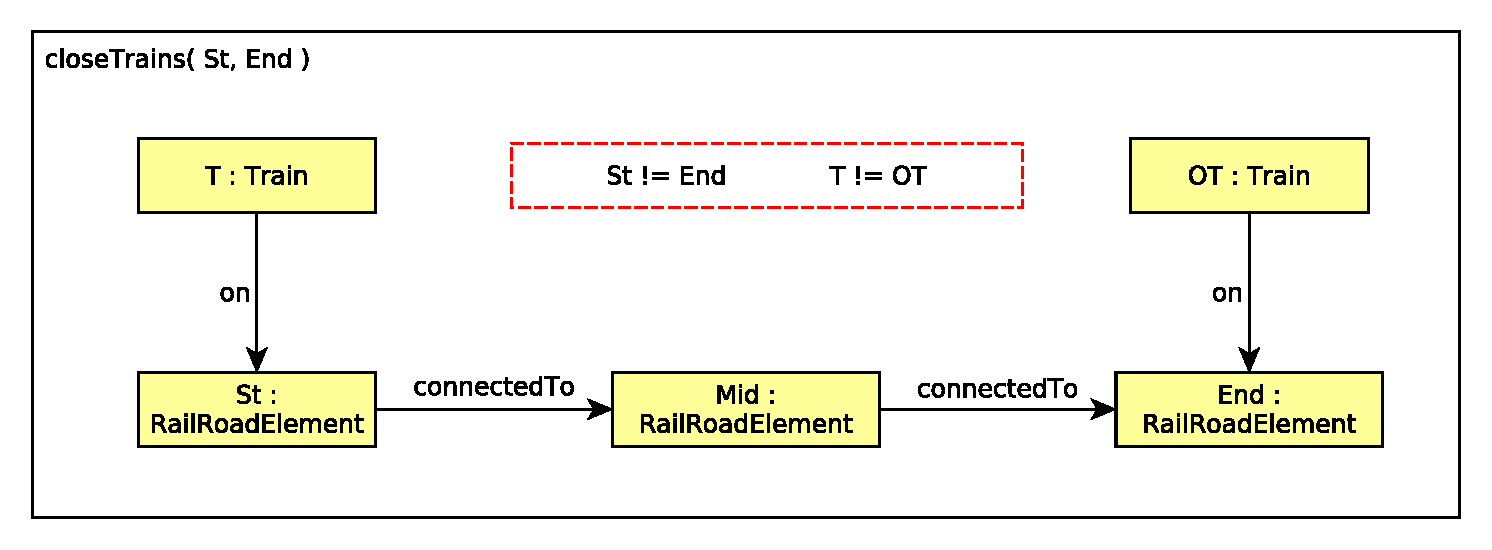
\includegraphics[width=\textwidth]{figures/closeTrains-pattern.pdf}
			\end{minipage}
			\hfill
			\begin{minipage}[c]{0.45\textwidth}
\begin{lstlisting}[language=vql]
pattern CloseTrains(St, End) {
	Train.on(T,St);
	Train.on(OT, End);
	RailRoadElement.connectedTo(St,Mid);
	RailRoadElement.connectedTo(Mid, end);
	T != OT;
	St != End;
}
\end{lstlisting}			
			\end{minipage}
			\hfill
			\begin{minipage}[l]{0.45\textwidth}
				
\begin{equation*}
\begin{array}{@{}l@{}}

\text{CloseTrains}(St, End) = \\
\exists{T} \  \exists{OT}\; \exists{Mid} ( \\
\text{on}(T, St)  \  \wedge \\
\text{on}(OT, End)  \  \wedge \\
\text{connectedTo}(St, Mid)  \  \wedge \\
\text{connectedTo}(Mid, End)  \  \wedge \\
\text{T} \neq OT  \  \wedge \\
\text{St} \neq End )
\end{array}
\end{equation*}
			
			\end{minipage}
		\end{minipage}
		\caption{CloseTrains pattern visualised (top), as defined in VQL (bottom left) and as a first-order logic expression (bottom right)}
		\label{fig:pattern-visual}
	\end{center}
\end{figure}



\section{Local search-based graph pattern matching}

Local search refers to a family of algorithms solving problems involving a search space. 
Local search starts from a candidate solution for a problem, then searches by applying local changes: moving to better neighboring solutions until eligible solutions are found.

Local search can also be used to find a match set for a graph pattern in a graph.
It is also a memory-efficient alternative for RETE algorithm in \viatra{}~\cite{bur-marton-msc}.
In our system, we use local search-based graph pattern matching. 

We define \emph{pattern body} as a subexpression of the graph pattern which has the following structure:
\begin{equation*}
\begin{array}{@{}c@{}}
\exists{\bar{x}} 
(\text{Constr}_{11}(\bar{p},\bar{x} ) \, \wedge \, 
 \text{Constr}_{12}(\bar{p},\bar{x} ) \, \wedge \, \dots{})
\end{array}
\end{equation*}
where $\bar{p}$ is the list of parameters, $\bar{v}$ is the list of variables that occur in the constraints.

In the following, we only use graph patterns composed by pattern bodies using the \emph{or} logical connective

\begin{equation*}
\begin{array}{@{}r@{}l@{}l@{}l@{}l@{}}
Pattern(p1, p2, \dots) = \;
& \exists{\bar{x}} ( & 
(\text{Constr}_{11}(\bar{p},\bar{x} ) & \, \wedge \, \text{Constr}_{12}(\bar{p},\bar{x} ) & \, \wedge \, \dots{}) \: \vee \\

& \exists{\bar{y}} & 
(\text{Constr}_{21}(\bar{p},\bar{y} ) & \, \wedge \, \text{Constr}_{22}(\bar{p},\bar{y} ) & \, \wedge \, \dots{}) \: \vee \\
& \dots{}
\end{array}
\end{equation*}

As VQL permits only this structure, the user must give the patterns in this form. This can be achieved by different transformations of the pattern, such as extracting negated expressions to subpatterns  and use negative pattern match constraint instead.

We can find the match set of this expression, by finding the match sets of all the pattern bodies as distinct predicates on the parameters, and taking their union.
The problem now is the following: find all variable bindings, which satisfies the constraints of the body.

\emph{Matching frame} of a body is defined as a partial function from variables to the domain of the graph i.e.\ as a partial variable binding.
A variable is bound in the frame, if it is mapped to a value, otherwise it is unbound.

Then the algorithm is the following:
\begin{enumerate}
	
\item
Let $C = (C_1, C_2, \dots{}, C_n )$ be the list of constraints in a given order.

\item 
Construct the frame, where all of the variables are unbound.

\item 
Starting from the first constraint:
	\begin{enumerate}
		\item 
		If all of the variables occurring in the constraint are bound in the current frame, then check if these values satisfies the constraint. 
		\begin{itemize}
			\item If they satisfy, then continue with the next constraint. If there are no more constraint, project this frame to the parameters and add it to the \mbox{match set}.
			\item if not, backtrack.
		\end{itemize}
		
		\item 
		If some variable occurring in the constraint are unbound, find all the possible values, that satisfy the constraints.
		Construct a frame for each of them, and continue for each frame at the next constraint. If there are no more constraints, project this frame to the parameters and add it to the match set.	
	\end{enumerate}	
\end{enumerate}
	
	
\begin{figure}[h]
	\begin{center}
		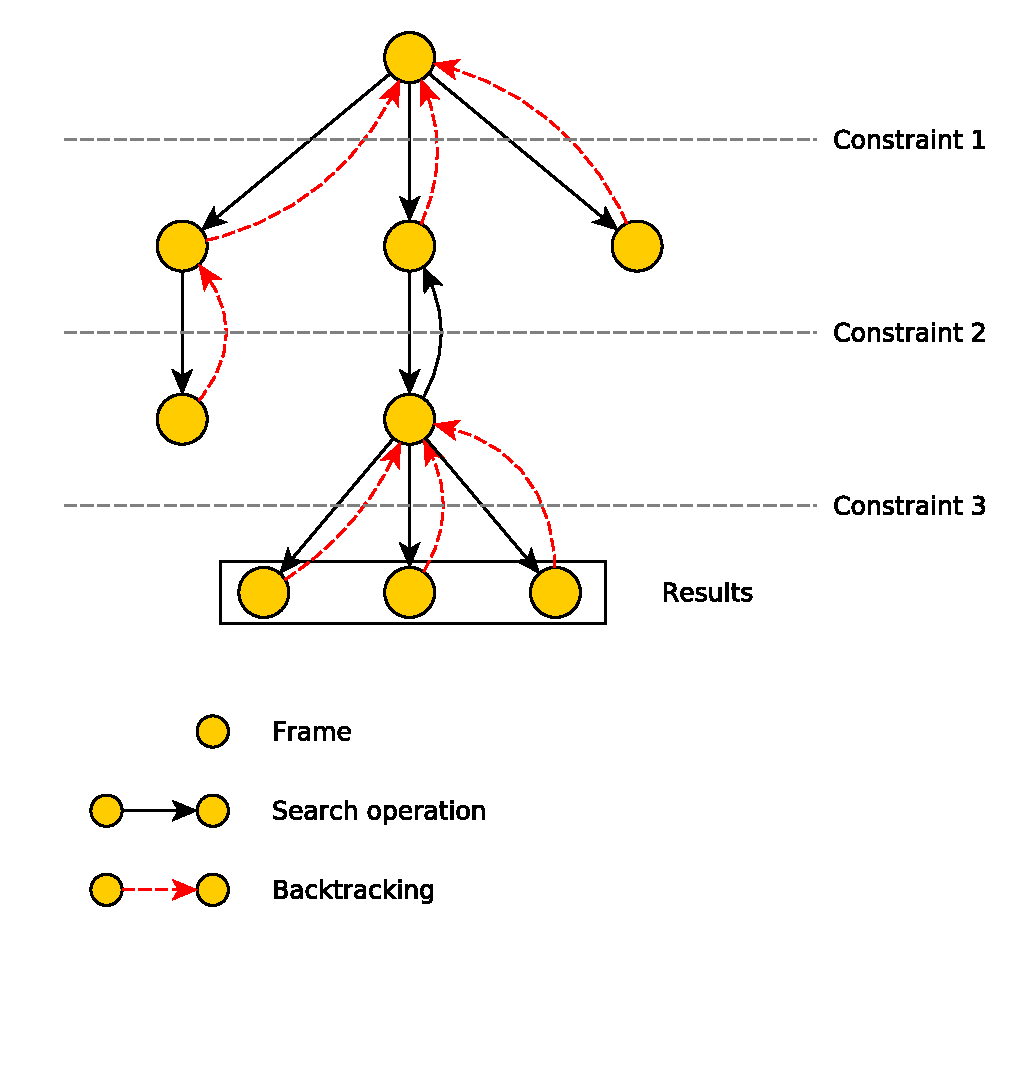
\includegraphics[width=0.7\textwidth]{figures/localsearch.pdf}
		\caption{Handling distributed models and cross-references}
		\label{fig:localsearch}
	\end{center}
\end{figure}
	
This algorithm is depicted in \autoref{fig:localsearch}. 
We can see, that it is a depth-first search in the space of frames. 
Because already bound variables are not modified, we can conclude the following:
\begin{itemize}
	\item 
	The search space is a tree, because all of the children of a frame will bind a variable differently, and these values are not changed in the subtree.
	\item
	At the $i$th layer of the tree, the first $i$ constraint is satisfied by the frame, as a child node does not modify already bound variables.
		
\end{itemize}

This means, that after computing the last constraint, the variable binding satisfies all the constraints, so it can be projected to the variables to form a solution.

We use depth-first search, because it uses less memory. Also generating depth-first search code is easy and efficient, as the layers are well defined. This way search can be easily implemented using nested for loops.

\subsection{Local search plan}
With a given order of the constraints, at the evaluation of the $i$th constraint we know what variables are already bound. Thus we know what kind of operation we will have to execute to generate the next frame which will satisfy the constraint.

A \emph{search operation} is an operation, that constructs the frames from the current frame, so they satisfy a given constraint.
\begin{itemize}
	\item 
	A \emph{check operation} is a search operation, which checks, whether the frame satisfies the given constraint. If it is, then the next frame is the same as the current frame, otherwise there are no next frames. (see the algorithm at 3.(a))
	\item
	An \emph{extend operation} is a search operation, which construct the next frames as all the frame, that binds the unbound variables which occurs in the constraint in a way, that the constraints is satisfied. (see the algorithm at 3.(b))

\end{itemize}


\emph{Local search plan} is a sequence of search operations.

\section{Distributed computational platform}

% adatok diszjunkt halmazokra bontva különböző csomópontra
% az algoritmusok is elosztottak, nem lesz összegyűjtve az infó, úgy van kiértékelve, hogy nincs aki mindent látna a rendszerből

In this thesis, the phrase \emph{computing unit} is used to denote a physical or virtual execution component of the CPS that is capable of storing a part of the graph model and updates it to represent the current state of the physical world, eg.\ an embedded system or a virtual machine.

In distributed CPSs various sensors serve as data sources and these sensors are connected to different computing units of the platform. However, in order to be able to monitor the distributed system as a whole, computing units need to exchange data.
Sending the sensor data to one computing unit and evaluate on that can cause different problems: 
sensor data can be too large to be sent over network, the central node can be a SPOF~(Single Point of Failure), etc. 

In the presented framework the live model is distributed into the different computing units and the graph pattern matching algorithm itself runs in a distributed way. 
This eliminates the problem of central computers, but introduces complexity, that we must handle.
One of the problems is distributed model handling, and the other is how to execute queries efficiently on a distributed platform.




\begin{figure}[h]
	\begin{center}
		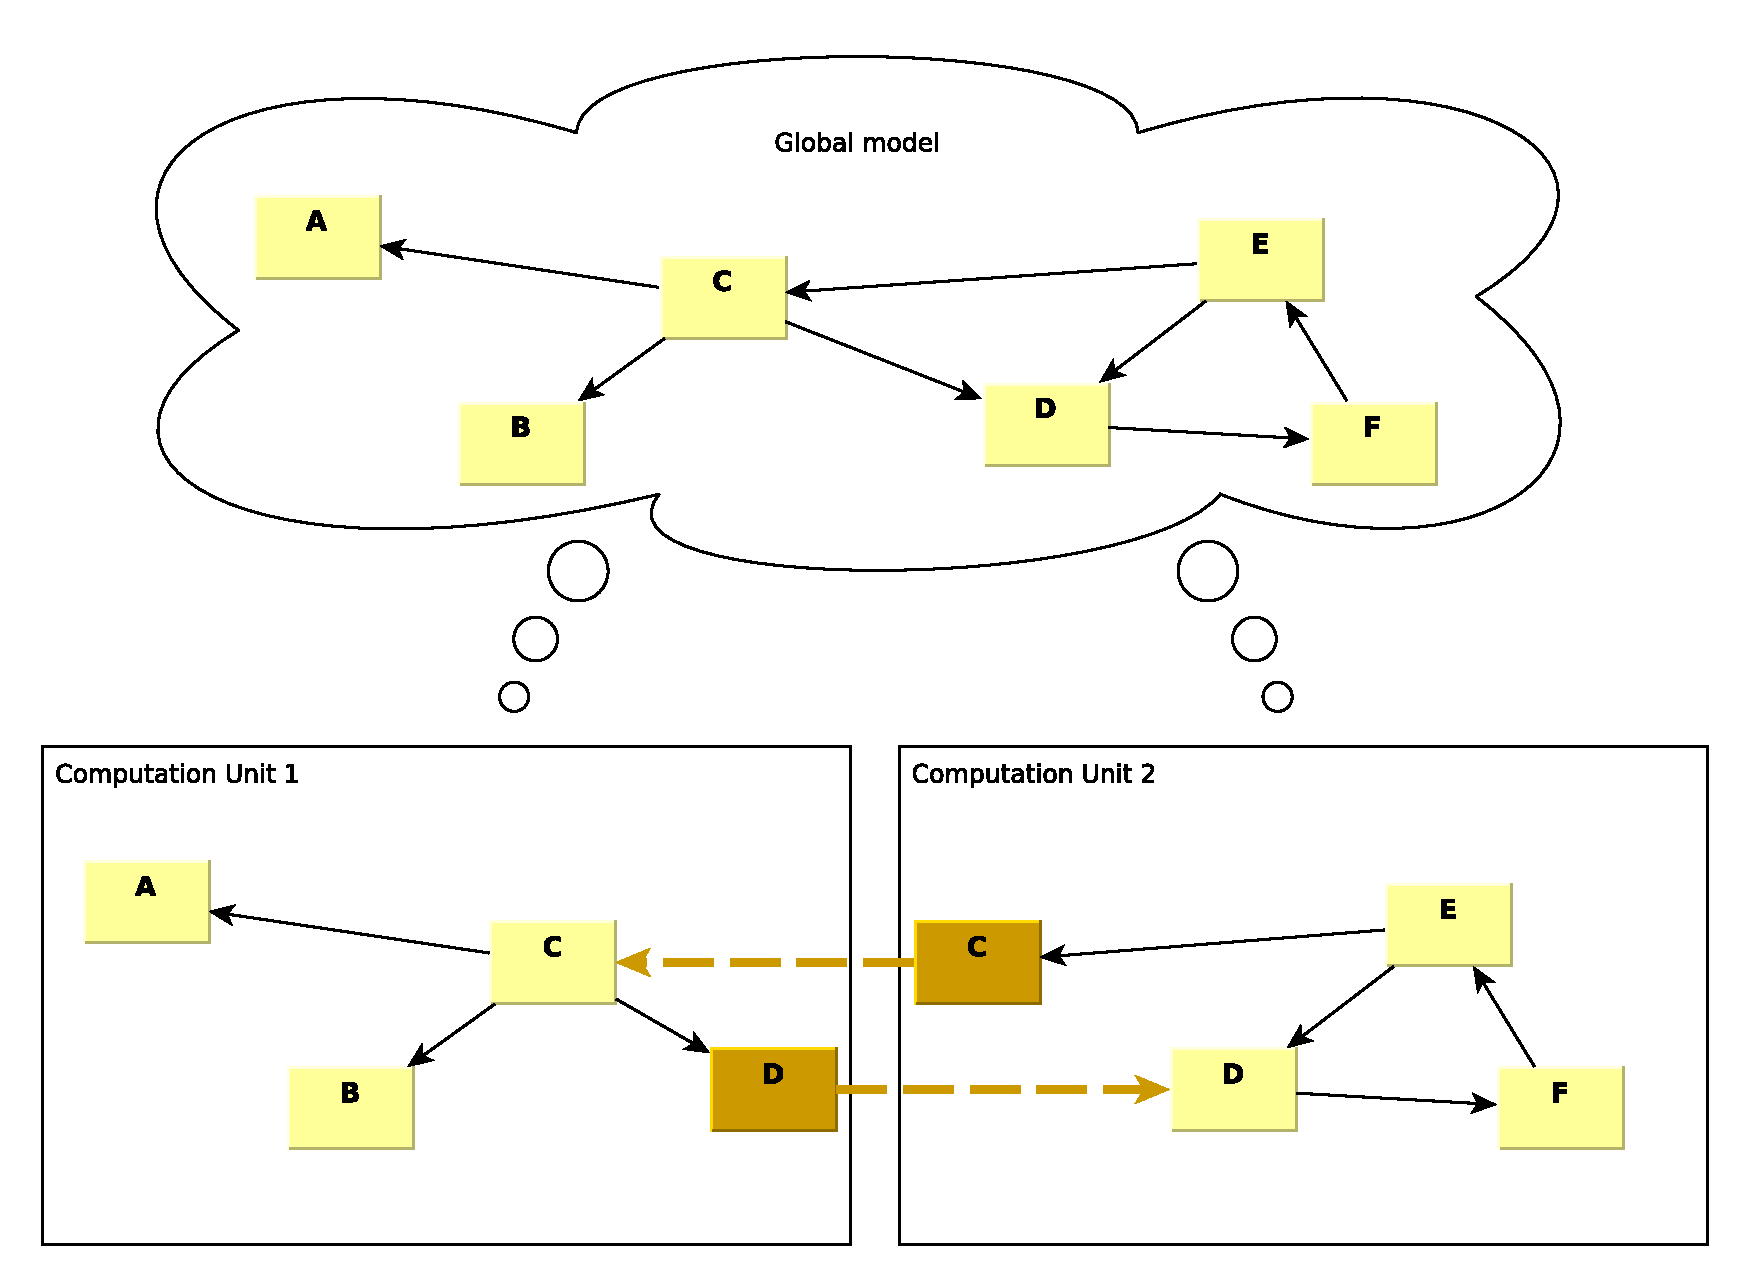
\includegraphics[width=\textwidth]{figures/distributed-model-handling.pdf}
		\caption{Handling distributed models and cross-references}
		\label{fig:distributed-model-handling}
	\end{center}
\end{figure}

\subsection{Distributed graph models}

In our framework each node in the graph is allocated to a computing unit. 
On that computing units, the node is called a \emph{local node}. 
In the context of other computing modules it is called a \emph{remote node}. 
Edges are stored in the computing module of their source node; 
If their target node is not a local node on that node, a \emph{proxy node} is used to substitute the remote node.
These concepts are illustrated in \autoref{fig:distributed-model-handling}.
From the perspective of Computing Unit 1, the green elements are local, and a red ones are remote. The yellow D is a proxy object which is used to represent the remote node in the reference from C to D.
A global model does not exist but computing units store partial models. Edges connecting elements of different computing units are stored by creating proxy elements on the computing unit of the source nodes. 


\subsection{Distributed query execution}

Distributed query execution is used in the framework to provide graph pattern matches
The purpose of distributed query execution is to run queries on distributed models on multiple computers. 
This introduces complexity, as we need to minimize network load, find matches that can span over multiple model parts, and provide low response times despite the distributed structure of the model.


\begin{figure}[h]
	\begin{center}
		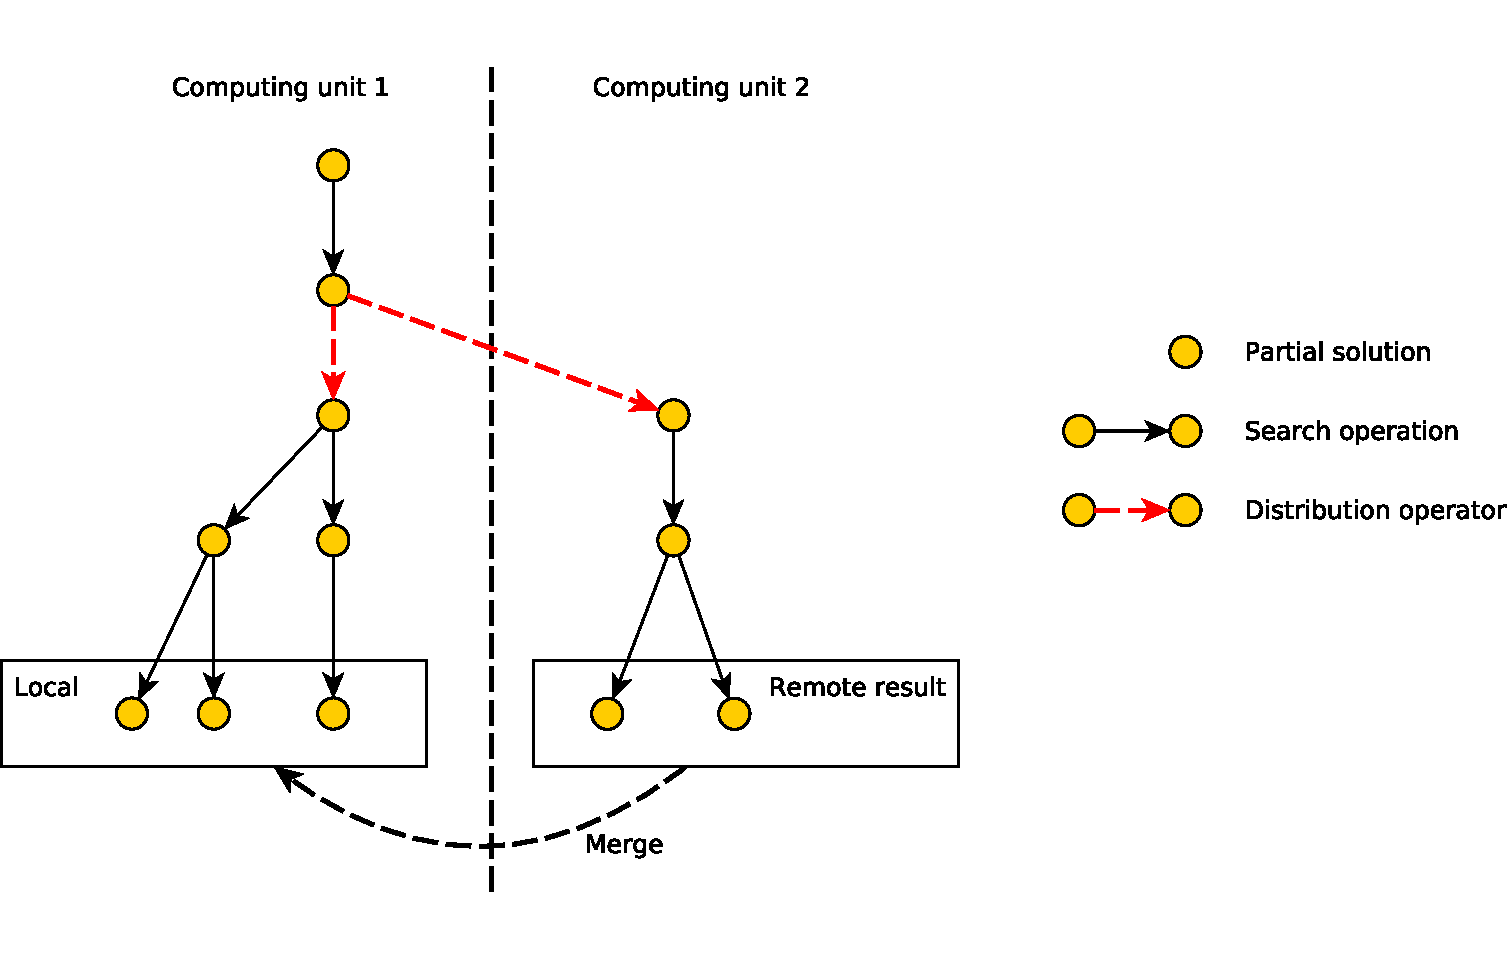
\includegraphics[width=\textwidth]{figures/distributed-ls.pdf}
		\caption{Distributed local search}
		\label{fig:distributed-ls}
	\end{center}
\end{figure}

In the framework, we extended local search-based graph pattern matching to work on distributed models.
This is achieved by doing the basic search operations locally, but create additional operations, which works in a distributed manner. 
Their mechanism is depicted on \autoref{fig:distributed-ls}.
These operations transmit the query execution to other computing units.
The other units continue to execute the query locally. When their results are calculated, they send it back to the caller.
The caller waits for the results and merges the local and remote results.

In this framework, we introduce two distributed operations:
\begin{itemize}
	\item Global distribution: globally distributes the query execution to all computing units (broadcast mechanics).
	\item Targeted distribution, distributes the query execution to the node, which contains a given model element.
\end{itemize}

The first can be used to globally iterate throw all elements of a given type. 
The latter is to help navigation through references, as references are stored locally.

A distributed local search plan can be calculated from a non-distributed one by the following:
\begin{itemize}
	\item If a search operation is based on reference constraint, we insert a targeted distribution operation before it to transmit the evaluation to the computing element containing the source variable.
	\item If a search operation is based on reference constraint, we insert global distribution operation before it to transmit the evaluation to all of the nodes, as any node can contain an object of that type.
\end{itemize}

This way, the distributed local search plan will have the same effect, but can be evaluated over distributed systems.


\section{Related work}

\newcommand{\mrt}{models\-@ run\-time\space}

In this section, the related work is summarized. The basis of this work has been published in \cite{FASE}, this related work is also based on that paper. Three main areas are related to the introduced approach: runtime verification, runtime verification of distributed systems and distributed graph query processing. All the related approaches are summarized in the following.

%TODO mindenhol legyen meg, hogy latszodjon, mi az uj
%\paragraph{Runtime verification approaches.}
\subsubsection{Runtime verification approaches}
For continuously evolving and dynamic CPSs, an upfront design-time formal analysis needs to incorporate and check the robustness of component behavior in a wide range of contexts and families of configurations, %\cite{Lee2014}, 
which is a very complex challenge. Thus consistent system behavior is frequently ensured by runtime verification (RV) \cite{Leucker2009}, which checks (potentially incomplete) execution traces against formal specifications by synthesizing verified runtime monitors from provenly correct design models \cite{Mitsch2014,Joshi2017}.

\subsubsection{Runtime verification of distributed systems}
While there are several existing techniques for runtime verification of sequential programs available, the authors of \cite{Mostafa2015} claim that much less research was done in this area for distributed systems. Furthermore, they provide the first sound and complete algorithm for runtime monitoring of distributed systems based on the 3-valued semantics of LTL.

\subsubsection{Distributed graph queries}
%TODO ezzel kapcsolatos eredmenyeket keresni
%TODO trinity
Highly efficient techniques for local-search based \cite{icgt2015} and incremental model queries \cite{scp2015} as part of the VIATRA framework were developed, which mainly builds on RETE networks as baseline technology. In \cite{models2014-iqd}, a distributed incremental graph query layer deployed over a cloud infrastructure with numerous optimizations was developed. 
Distributed graph query evaluation techniques were reported in \cite{Mitschke2014,Peters2014,Krause2014}, but none of these techniques considered an execution environment with resource-constrained computation units.

\subsubsection{Runtime models} 
The \mrt paradigm~\cite{DBLP:journals/computer/BlairBF09} serves as the conceptual basis for the Kevoree framework~\cite{Morin2014} (developed within the HEADS FP7 project). Other recent distributed, data-driven solutions include the Global Data Plane \cite{Zhang2015} and executable metamodels at runtime \cite{Vogel2014}. However, these frameworks currently offer very limited support for efficiently evaluating queries over a distributed runtime platform, which is the main focus of our current work.







